% -*- coding: utf-8 -*-

\chapter{相关理论与技术背景} \label{chpt:background}

本章系统介绍本文研究所涉及的核心理论与技术背景，主要包括四个方面：深度神经网络的基础知识、对抗样本与对抗攻击方法、对抗性训练框架，以及像素重要性分析方法。这四个方面共同构成了本文方法设计与实验分析的理论基础。

\section{深度神经网络基础}

\subsection{卷积神经网络}

卷积神经网络（Convolutional Neural Network，CNN）是深度学习领域最具影响力的模型架构之一，在图像分类、目标检测、语义分割等计算机视觉任务中取得了突破性进展\cite{lecun2015deeplearning,krizhevsky2012imagenet}。与传统的全连接神经网络相比，卷积神经网络通过局部连接和权重共享机制，极大地降低了参数量，同时利用卷积核自动提取图像的局部空间特征，具有平移不变性。

卷积神经网络一般由卷积层、池化层和全连接层三类核心层组成。

\textbf{卷积层}是CNN的核心组成部分，其基本操作是将一个可学习的滤波器与输入特征图作局部点积运算。设输入特征图为 $\mathbf{X} \in \mathbb{R}^{H \times W \times C_{in}}$，卷积核为 $\mathbf{W} \in \mathbb{R}^{k \times k \times C_{in}}$，偏置为 $b$，则第 $(i, j)$ 位置的输出特征值为：

\begin{equation}
  y_{i,j} = \sum_{m=0}^{k-1} \sum_{n=0}^{k-1} \sum_{c=1}^{C_{in}} W_{m,n,c} \cdot X_{i+m,\, j+n,\, c} + b
\end{equation}

其中 $k$ 为卷积核大小，$C_{in}$ 为输入通道数。通过引入多个卷积层，网络可以提取从低级边缘、纹理到高级语义等特征。

\textbf{激活函数}为神经网络引入非线性变换，使网络能够拟合复杂的非线性函数关系。修正线性单元（Rectified Linear Unit，ReLU）是目前最广泛使用的激活函数，其定义为：

\begin{equation}
  \text{ReLU}(x) = \max(0, x)
\end{equation}

ReLU函数计算简单，能有效缓解深层网络训练中的梯度消失问题，加快训练收敛速度。

\textbf{池化层}对特征图进行下采样，降低特征维度，同时增强模型对微小位置变化的鲁棒性。最大池化操作在每个局部窗口内取最大值，是最常用的池化操作。设池化窗口大小为 $p \times p$，步长为 $s$，则：

\begin{equation}
  z_{i,j} = \max_{0 \le m < p,\; 0 \le n < p} y_{i \cdot s + m,\; j \cdot s + n}
\end{equation}

\textbf{全连接层}将卷积层提取到的特征展平后进行线性变换，通常位于网络末端，完成最终的分类或回归任务。

\subsection{LeNet-5网络结构}

LeNet-5是由LeCun等人提出的经典卷积神经网络架构\cite{lecun1998lenet}，最初用于手写数字识别任务，是现代CNN架构的重要先驱，其网络结构如图\ref{fig:lenet5}
所示。
\begin{figure}[htbp]
    \centering
    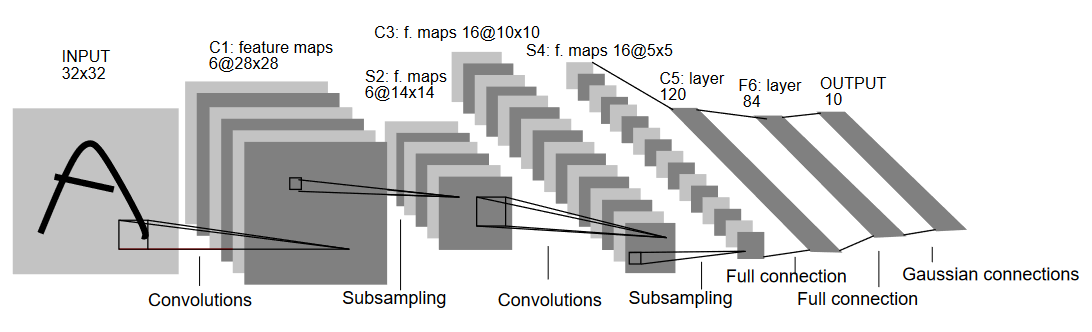
\includegraphics[width=0.9\textwidth]{figures/lenet5.png}
    \caption{LeNet-5网络结构示意图}
    \label{fig:lenet5}
\end{figure}

本文所使用的LeNet-5网络结构在原始架构基础上进行了适配调整，以更好地适配MNIST数据集（$28 \times 28$ 灰度图像，10类）。输入图像首先经过均值为0.1307、标准差为0.3081的归一化处理，以加速训练收敛，并提升神经网络泛化能力。第一卷积层使用 $\text{padding}=2$ 以保持输入的空间尺寸不变，使 $28\times28$ 的输入经过 $5\times5$ 卷积后仍保持 $28\times28$，再经 $2\times2$ 最大池化降采样为 $14\times14$；第二卷积层不使用填充，将特征图从 $14\times14$ 降至 $10\times10$，再经池化降为 $5\times5$；最终将 $16\times5\times5=400$ 维特征展平后依次经过三个全连接层，输出10类对数概率。网络各层的详细配置如表\ref{tab:lenet5}所示。

\begin{table}[htbp]
  \centering
  \caption{本文使用的LeNet-5网络结构}
  \label{tab:lenet5}
  \begin{tabular}{lllll}
    \toprule
    层次编号 & 层类型 & 配置参数 & 激活函数 & 输出尺寸 \\
    \midrule
    输入 & 归一化层 & mean=0.1307，std=0.3081 & — & $1 \times 28 \times 28$ \\
    1 & 卷积层 & $1 \to 6$，核$5\times5$，padding=2 & ReLU & $6 \times 28 \times 28$ \\
    1 & 最大池化 & $2\times2$，stride=2 & — & $6 \times 14 \times 14$ \\
    2 & 卷积层 & $6 \to 16$，核$5\times5$ & ReLU & $16 \times 10 \times 10$ \\
    2 & 最大池化 & $2\times2$，stride=2 & — & $16 \times 5 \times 5$ \\
    3 & 全连接层 & $400 \to 120$ & ReLU & $120$ \\
    4 & 全连接层 & $120 \to 84$ & ReLU & $84$ \\
    5 & 全连接层 & $84 \to 10$ & — & $10$ \\
    \bottomrule
  \end{tabular}
\end{table}

\subsection{损失函数与优化}

在分类任务中，交叉熵损失函数（Cross-Entropy Loss）是最常用的目标函数。设模型对样本 $\mathbf{x}$ 输出的类别概率分布为 $\mathbf{p} = \text{softmax}(f_\theta(\mathbf{x}))$，真实标签为 $y$，则交叉熵损失定义为：

\begin{equation}
  \mathcal{L}_{CE}(\mathbf{x}, y;\, \theta) = -\log p_y = -\log \frac{\exp\!\left(f_\theta(\mathbf{x})_y\right)}{\displaystyle\sum_{j=1}^{K} \exp\!\left(f_\theta(\mathbf{x})_j\right)}
\end{equation}

其中 $K$ 为类别总数，$f_\theta(\mathbf{x})_j$ 为第 $j$ 类的输出 logit 值。最小化交叉熵损失等价于最大化模型对真实类别的预测概率。

在优化算法方面，本文采用Adam优化器\cite{kingma2015adam}训练网络参数。Adam结合了动量（Momentum）和自适应学习率（RMSProp）的优势，对梯度的一阶矩和二阶矩分别进行指数移动平均估计，在不同任务和网络结构上均表现出良好的收敛性和鲁棒性，是深度学习训练中应用最为广泛的优化算法之一。

\section{对抗样本与对抗攻击}

\subsection{对抗样本的定义}

对抗样本（Adversarial Examples）是指在原始输入样本 $\mathbf{x}$ 的基础上，通过添加人眼难以察觉的微小扰动 $\boldsymbol{\delta}$，生成一个能够欺骗深度神经网络产生错误预测的输入 $\mathbf{x}' = \mathbf{x} + \boldsymbol{\delta}$。Szegedy等人在2014年首次系统性地发现并研究了这一现象\cite{szegedy2014intriguing}，指出即便是在分类任务上表现优异的深度神经网络，也对精心设计的微小输入扰动极为敏感。

形式化地，给定分类器 $f: \mathcal{X} \to \mathcal{Y}$ 和输入样本 $\mathbf{x}$（真实标签为 $y_{true}$），对抗样本 $\mathbf{x}'$ 需同时满足以下两个条件：

\begin{equation}
  f(\mathbf{x}') \neq y_{true} \quad \text{且} \quad d(\mathbf{x},\, \mathbf{x}') < \varepsilon
\end{equation}

其中 $d(\cdot, \cdot)$ 为度量扰动大小的距离函数，$\varepsilon > 0$ 为扰动预算（perturbation budget），控制对抗扰动的幅度上限。

根据 $d(\cdot, \cdot)$ 的选取方式，常见的扰动度量有以下三种范数：

\textbf{$L_\infty$ 范数}：$\|\boldsymbol{\delta}\|_\infty = \max_i |\delta_i|$，约束每个像素的扰动幅度均不超过 $\varepsilon$，是FGSM、PGD等主流攻击方法采用的扰动度量，适合描述分布在全局的均匀微小扰动。

\textbf{$L_2$ 范数}：$\|\boldsymbol{\delta}\|_2 = \sqrt{\sum_i \delta_i^2}$，约束整体扰动的欧氏距离，适合描述全局细微的扰动。C\&W攻击等方法以此为优化目标。

\textbf{$L_0$ 范数}：$\|\boldsymbol{\delta}\|_0 = \left|\{i : \delta_i \neq 0\}\right|$，统计被修改的像素数量，允许对少数像素施加较大幅度的扰动，其余像素保持不变。$L_0$ 范数约束与本文所研究的遮蔽攻击（Occlusion Attack）类似，遮蔽攻击同样只对图像的局部区域施加较强干预，其本质可视为 $L_0$ 范数约束下的一种极端扰动形式。

\subsection{基于梯度的对抗攻击方法}

\subsubsection*{FGSM攻击}

快速梯度符号法（Fast Gradient Sign Method，FGSM）由Goodfellow等人提出\cite{goodfellow2015fgsm}，是最具代表性的单步对抗攻击方法。FGSM利用损失函数关于输入的梯度方向构造对抗扰动，其生成公式为：

\begin{equation}
  \mathbf{x}' = \mathbf{x} + \varepsilon \cdot \text{sign}\!\left(\nabla_{\mathbf{x}}\, \mathcal{L}(f(\mathbf{x}), y)\right)
\end{equation}

其中 $\text{sign}(\cdot)$ 为符号函数，$\varepsilon$ 为扰动步长。FGSM沿使损失函数增大最快的方向对每个像素施加大小为 $\varepsilon$ 的扰动，一步生成对抗样本，计算效率极高，但由于单步近似粗糙，攻击强度相对有限。

\subsubsection*{PGD攻击}

投影梯度下降攻击（Projected Gradient Descent，PGD）由Madry等人提出\cite{madry2018pgd}，是FGSM的多步迭代扩展，也是目前最为重要的对抗攻击基准之一。PGD在 $\varepsilon$-球约束集内反复执行梯度上升步骤，并在每步之后将扰动投影回约束集：

\begin{equation}
  \mathbf{x}^{(t+1)} = \Pi_{\mathcal{B}_\varepsilon(\mathbf{x})} \!\left( \mathbf{x}^{(t)} + \alpha \cdot \text{sign}\!\left(\nabla_{\mathbf{x}}\, \mathcal{L}(f(\mathbf{x}^{(t)}), y)\right) \right)
\end{equation}

其中 $\alpha$ 为每步步长，$\Pi_{\mathcal{B}_\varepsilon(\mathbf{x})}$ 表示投影到以 $\mathbf{x}$ 为中心、半径为 $\varepsilon$ 的 $L_\infty$ 球上的投影算子，初始扰动 $\mathbf{x}^{(0)}$ 通常在约束集内随机初始化。PGD通过多步迭代能够更充分地搜索对抗扰动空间，攻击强度显著高于FGSM，是评估模型鲁棒性的标准基准攻击。

\subsubsection*{C\&W攻击}

Carlini和Wagner提出的C\&W攻击\cite{carlini2017cw}将对抗样本生成转化为连续优化问题，通过最小化以下目标函数来寻找扰动幅度尽可能小的高置信度对抗样本：

\begin{equation}
  \min_{\boldsymbol{\delta}} \;\|\boldsymbol{\delta}\|_2 + c \cdot g(\mathbf{x} + \boldsymbol{\delta})
\end{equation}

其中 $g(\cdot)$ 是以分类置信度为基础构造的攻击目标函数，当 $\mathbf{x}+\boldsymbol{\delta}$ 被错误分类时取负值，$c > 0$ 为平衡扰动幅度与攻击成功率的超参数。C\&W攻击能够在 $L_2$ 约束下生成人眼极难察觉的高质量对抗样本，常被用作攻击强度的参照基准，可绕过许多基于梯度掩盖的防御方法。

\subsection{基于遮蔽的对抗攻击}

与基于 $L_p$ 范数约束的梯度攻击方法不同，基于遮蔽的对抗攻击（Occlusion-based Adversarial Attack）通过在图像的局部区域施加大幅度修改（如将像素值设为固定颜色、纯黑或噪声块）来欺骗分类器，其本质是对少数像素实施"局部大幅扰动"而非"全局均匀小幅扰动"。这类攻击的核心思想在于：并非所有像素对模型决策的贡献都相同——模型倾向于依赖少数关键区域做出判断，若这些关键区域被遮蔽或替换，模型极易产生错误预测。

基于遮蔽的对抗攻击与物理世界中的真实威胁场景高度契合。Brown等人提出的对抗性贴片（Adversarial Patch）\cite{brown2017adversarialpatch}通过在图像中放置一块可打印的对抗性图案，无论贴片放置在何位置，均能使分类器产生目标误分类，且该方法在物理打印环境下仍具有可迁移性。Eykholt等人\cite{eykholt2018robust}进一步将遮蔽攻击应用于道路标志识别场景，通过在停车标志上粘贴特定图案，成功使自动驾驶系统的视觉识别模型产生严重误判，揭示了此类攻击在安全关键领域的现实威胁性。

基于遮蔽攻击的上述特点，本文结合显著性图方法，设计了针对关键语义区域的遮蔽攻击策略，并以此为基础构建对抗性训练方法，具体内容将在第3章详细阐述。

\section{对抗性训练}

\subsection{对抗性训练的基本框架}

对抗性训练（Adversarial Training）是目前被认为最有效的对抗防御方法之一，其核心思想是在模型训练过程中引入对抗性样本进行训练，使模型通过接触多样化的对抗扰动来增强自身鲁棒性。

对抗性训练的优化目标可形式化为一个min-max鞍点优化问题\cite{madry2018pgd}：

\begin{equation}
  \min_{\theta} \; \mathbb{E}_{(\mathbf{x}, y) \sim \mathcal{D}} \left[ \max_{\boldsymbol{\delta} \in \mathcal{S}} \mathcal{L}(f_\theta(\mathbf{x} + \boldsymbol{\delta}),\, y) \right]
\end{equation}

其中 $\mathcal{D}$ 为训练数据分布，$\mathcal{S}$ 为允许的扰动集合（如 $L_\infty$ 球 $\mathcal{B}_\varepsilon$），$\theta$ 为网络参数。该双层优化问题包含两个嵌套的优化过程：

\textbf{内层最大化}：对每个训练样本 $(\mathbf{x}, y)$，在扰动约束集 $\mathcal{S}$ 内求解使损失最大化的对抗扰动 $\boldsymbol{\delta}^*$，等价于在当前模型参数下寻找最强的攻击；

\textbf{外层最小化}：使用内层攻击生成的对抗样本更新模型参数 $\theta$，使模型对最坏情况下的对抗扰动具有较低损失，从而提升鲁棒性。

Madry等人从鞍点优化角度对该框架进行了理论分析，并证明使用PGD攻击近似求解内层最大化问题，能够有效提升模型的 $L_\infty$ 鲁棒性\cite{madry2018pgd}。

\subsection{主要对抗性训练方法}

\subsubsection*{PGD对抗性训练（PGD-AT）与变体}

PGD对抗性训练（PGD-AT）是最经典的对抗性训练方法，在训练中，先通过多步PGD攻击生成当前样本的对抗样本，再以这些对抗样本计算损失并更新模型参数。该方法防御效果显著，但由于每个训练步骤需要执行多次前向和反向传播来生成对抗样本，训练开销是标准训练的数倍至数十倍。

为降低对抗性训练的计算开销，Wong等人提出了基于随机初始化FGSM的快速对抗性训练方法（FGSM-AT）\cite{wong2020fast}，通过单步FGSM攻击代替多步PGD生成对抗样本，将训练成本降低至接近标准训练的水平；Shafahi等人提出的Free对抗性训练\cite{shafahi2019free}则通过在单次前向-反向传播中同时更新扰动参数和模型参数，进一步提高了训练效率，在保持较好鲁棒性的同时大幅削减了计算成本。

\subsection{对抗性训练的局限性}

尽管对抗性训练已取得显著进展，但其在实际应用中仍面临以下主要局限：

\textbf{攻击类型专一性}：现有对抗性训练方法通常针对特定攻击类型（如 $L_\infty$-PGD）进行优化，对训练过程中未见的攻击类型（如 $L_2$ 攻击、遮蔽攻击）往往缺乏有效防御。模型在特定威胁模型下的鲁棒性提升并不能自动泛化到其他攻击形式，这是对抗性训练泛化性不足的核心问题，也是本文研究混合对抗性训练策略的重要动机。

\textbf{干净准确率下降}：引入对抗样本训练后，模型在干净测试样本上的准确率通常会出现不同程度的下降，即存在"鲁棒性—准确率权衡"（robustness-accuracy trade-off）现象。这一问题在实际部署中尤为突出，因为系统不仅需要抵御对抗攻击，也必须在正常输入上保持高精度。

\textbf{训练计算开销大}：以PGD-AT为代表的对抗性训练方法需要执行多步迭代攻击，导致训练时间远高于标准训练，在大规模数据集和复杂网络结构下，这一问题尤为突出，限制了对抗性训练的实际应用范围。

\section{像素重要性分析方法}

像素重要性分析（Pixel Importance Analysis）方法旨在量化输入特征对神经网络预测结果的贡献程度，并可视化模型的"注意力"分布。这类方法在模型可解释性研究中具有重要地位，同时也为本文的遮蔽攻击提供了关键区域定位的依据。

\subsection{原始梯度显著性图方法}

原始梯度显著性图（Vanilla Gradient  Saliency Map,Saliency Map）由Simonyan等人提出\cite{simonyan2014saliency}，是最基础也最直观的像素重要性分析方法。其核心思想是：模型预测对某一输入像素的梯度绝对值越大，说明该像素对预测结果的影响越大，即该像素越"显著"。

形式化地，设 $f_c(\mathbf{x})$ 为模型关于类别 $c$ 的输出分数，则输入 $\mathbf{x}$ 的显著性图定义为：

\begin{equation}
  \mathbf{S}(\mathbf{x}) = \left| \frac{\partial f_c(\mathbf{x})}{\partial \mathbf{x}} \right|
\end{equation}

其中 $|\cdot|$ 表示逐元素取绝对值。$\mathbf{S}(\mathbf{x})$ 的每个元素对应输入图像中相应像素的重要性得分，整体构成一张与输入图像等尺寸的显著性热力图，高值区域对应对模型决策贡献最大的像素位置。

Saliency Map的主要优势在于计算效率极高：只需对输入进行一次前向传播和一次反向传播即可获得完整的显著性图，无需对模型结构进行任何修改。在需要对每个训练样本实时计算Saliency Map的对抗性训练场景中，这一特性尤为重要。

\subsection{IG方法}

梯度积分（Integrated Gradients，IG）由Sundararajan等人提出\cite{sundararajan2017ig}，是一种在理论上更为严格的像素重要性分析方法。IG的核心思想是沿从基线输入 $\mathbf{x}^{(0)}$（通常为全零图像）到目标输入 $\mathbf{x}$ 的路径上对梯度进行积分，从而计算每个特征对预测变化的累积贡献：

\begin{equation}
  \text{IG}_i(\mathbf{x}) = \left(x_i - x^{(0)}_i\right) \cdot \int_0^1 \frac{\partial f_c\!\left(\mathbf{x}^{(0)} + \alpha\!\left(\mathbf{x} - \mathbf{x}^{(0)}\right)\right)}{\partial x_i} \, \mathrm{d}\alpha
\end{equation}

其中 $x_i$ 和 $x^{(0)}_i$ 分别为目标输入和基线输入第 $i$ 个特征的值，$\alpha \in [0, 1]$ 为插值参数。在实际计算中，连续积分通常被离散化为 $m$ 步黎曼和近似：

\begin{equation}
  \text{IG}_i(\mathbf{x}) \approx \left(x_i - x^{(0)}_i\right) \cdot \frac{1}{m} \sum_{k=1}^{m} \frac{\partial f_c\!\left(\mathbf{x}^{(0)} + \frac{k}{m}\!\left(\mathbf{x} - \mathbf{x}^{(0)}\right)\right)}{\partial x_i}
\end{equation}

积分梯度（IG）方法满足两个重要的公理性质：

\textbf{敏感性公理（Sensitivity）}：若两个输入仅在某一特征上不同，且模型输出不同，则该特征的像素重要性分析值应非零，确保像素重要性分析结果能够真实反映特征对预测的贡献；

\textbf{实现不变性公理（Implementation Invariance）}：对于任意两个功能等价的网络（即对所有输入具有相同输出），其像素重要性分析结果应相同，保证像素重要性分析方法的一致性，不受具体网络实现细节的影响。


\section{本章小结}

本章系统梳理了本文研究所依赖的核心理论与技术背景。首先介绍了卷积神经网络的基本组成与工作原理，阐述了LeNet-5的具体网络结构及其在MNIST任务上的适配方案，并介绍了交叉熵损失函数与Adam优化器。其次，详细介绍了FGSM、PGD、C\&W等主流基于梯度的对抗攻击方法，以及基于遮蔽的对抗攻击。第三，从min-max优化的视角阐述了对抗性训练的基本框架，介绍了PGD-AT、FGSM-AT和Free训练等主流方法，并分析了对抗性训练在攻击泛化性、干净准确率和计算开销方面的主要局限。最后，介绍了Saliency Map和IG两种像素重要性分析方法。
